\usepackage{booktabs}

\def\tightlist{}



%----------------------------------------------------------------%
%                          COPERTINA                             %
%----------------------------------------------------------------%

\makeatletter

\def\thickhrulefill{\leavevmode \leaders \hrule height 1pt\hfill \kern \z@}

\def\maketitle{%
  \null
  \thispagestyle{empty}%
  % scommentare se si vuole costruire l'eserciziario ( commentare la riga dopo)
  % \begin{flushleft}
\includegraphics[scale=.175]{exercises/images/quantide.png}\end{flushleft}
  \hspace{-2cm}
   \begin{flushleft}
\includegraphics[width=50mm]{./images/quantide.png}\end{flushleft}
  \vspace{-2cm}
  % scommentare se si vuole costruire l'eserciziario ( commentare la riga dopo)
  %\begin{flushright}
\includegraphics[scale=.25]{exercises/images/R-training.png}\end{flushright}
  \begin{flushright}
\includegraphics[width=20mm]{./images/Rlogo.png}\end{flushright}
  \vskip 3cm
  \hrule height 2pt
  \begin{center} \par \huge \strut \textbf{$My  First  Date  with  R$}\\ $Manual$ \par  \end{center}
  \vspace{0.5cm}
  \hrule height 2pt
  \vspace{0.5cm}
  \vspace{2cm}
  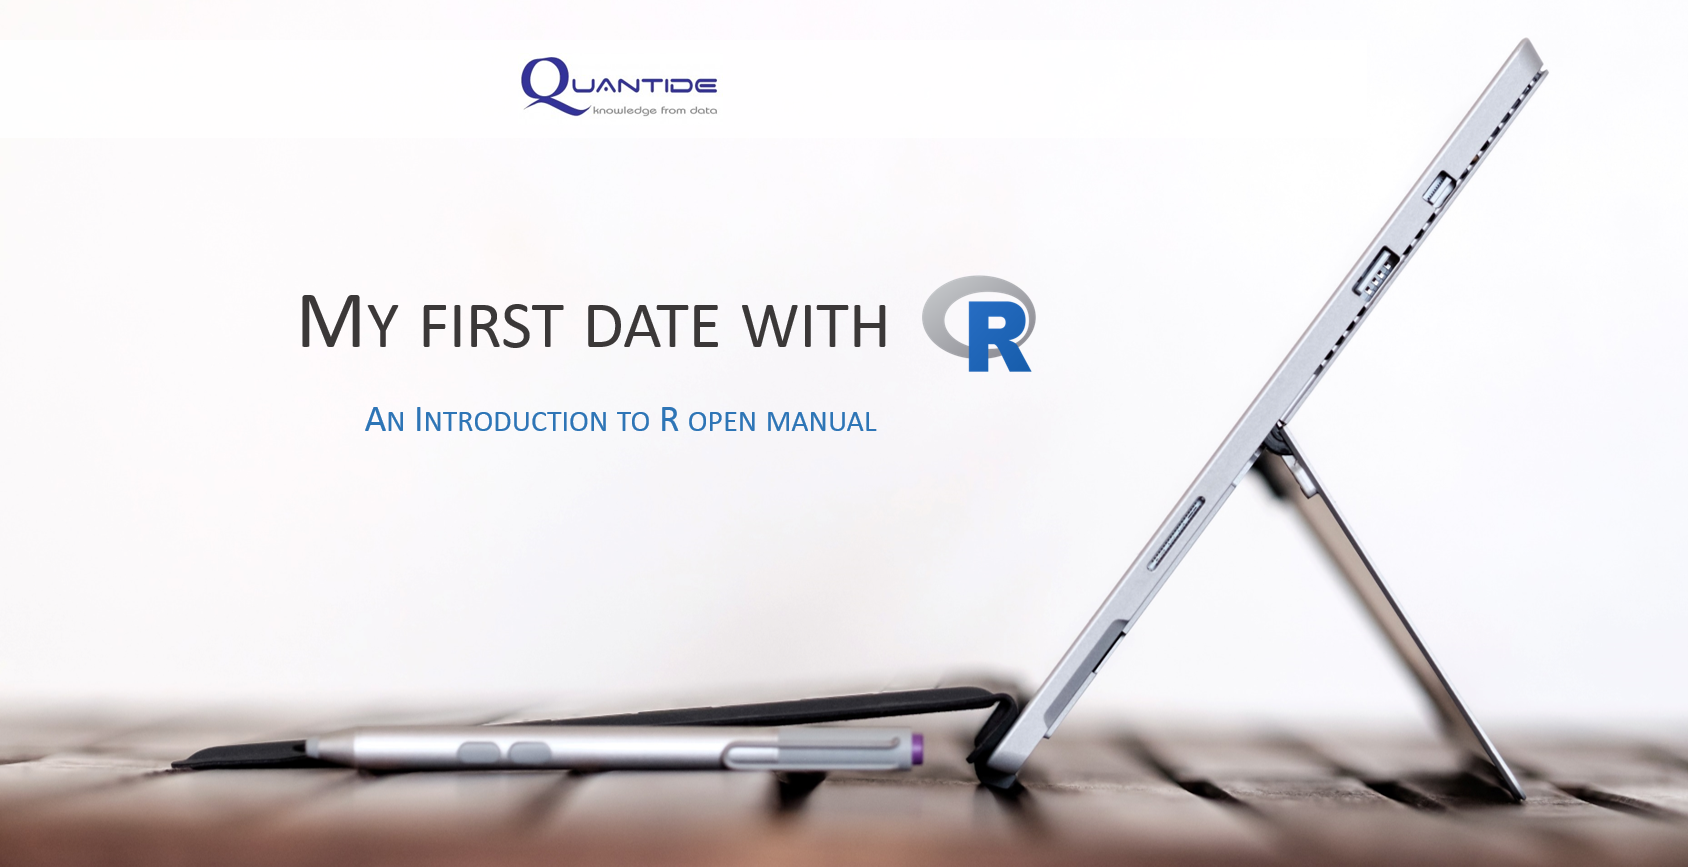
\includegraphics[width=165mm]{./images/Locandina_Florida_Banner.png}
  \clearpage
}

\makeatother
%----------------------------------------------------------------%






